%%%%%%%%%%%%%%%%%%%%%%%%%%%%%%%%%%%%%%%%%
% Arsclassica Article
% LaTeX Template
% Version 1.1 (10/6/14)
%
% This template has been downloaded from:
% http://www.LaTeXTemplates.com
%
% Original author:
% Lorenzo Pantieri (http://www.lorenzopantieri.net) with extensive modifications by:
% Vel (vel@latextemplates.com)
%
% License:
% CC BY-NC-SA 3.0 (http://creativecommons.org/licenses/by-nc-sa/3.0/)
%
%%%%%%%%%%%%%%%%%%%%%%%%%%%%%%%%%%%%%%%%%

%----------------------------------------------------------------------------------------
%	PACKAGES AND OTHER DOCUMENT CONFIGURATIONS
%----------------------------------------------------------------------------------------

\documentclass[
10pt, % Main document font size
letterpaper, % Paper type, use 'letterpaper' for US Letter paper
oneside, % One page layout (no page indentation)
%twoside, % Two page layout (page indentation for binding and different headers)
headinclude,footinclude, % Extra spacing for the header and footer
BCOR5mm, % Binding correction
]{scrartcl}

%%%%%%%%%%%%%%%%%%%%%%%%%%%%%%%%%%%%%%%%%
% Arsclassica Article
% Structure Specification File
%
% This file has been downloaded from:
% http://www.LaTeXTemplates.com
%
% Original author:
% Lorenzo Pantieri (http://www.lorenzopantieri.net) with extensive modifications by:
% Vel (vel@latextemplates.com)
%
% License:
% CC BY-NC-SA 3.0 (http://creativecommons.org/licenses/by-nc-sa/3.0/)
%
%%%%%%%%%%%%%%%%%%%%%%%%%%%%%%%%%%%%%%%%%

%----------------------------------------------------------------------------------------
%	REQUIRED PACKAGES
%----------------------------------------------------------------------------------------

\usepackage[
nochapters, % Turn off chapters since this is an article        
beramono, % Use the Bera Mono font for monospaced text (\texttt)
eulermath,% Use the Euler font for mathematics
pdfspacing, % Makes use of pdftex’ letter spacing capabilities via the microtype package
dottedtoc % Dotted lines leading to the page numbers in the table of contents
]{classicthesis} % The layout is based on the Classic Thesis style

\usepackage{arsclassica} % Modifies the Classic Thesis package

\usepackage[T1]{fontenc} % Use 8-bit encoding that has 256 glyphs

\usepackage[utf8]{inputenc} % Required for including letters with accents

\usepackage{graphicx} % Required for including images
\graphicspath{{Figures/}} % Set the default folder for images

\usepackage{enumitem} % Required for manipulating the whitespace between and within lists

\usepackage{lipsum} % Used for inserting dummy 'Lorem ipsum' text into the template

\usepackage{subfig} % Required for creating figures with multiple parts (subfigures)

\usepackage{amsmath,amssymb,amsthm} % For including math equations, theorems, symbols, etc

\usepackage{varioref} % More descriptive referencing

\usepackage{url}

\usepackage{listings}

\usepackage[numbers]{natbib} % required for cite author to work
%----------------------------------------------------------------------------------------
%	THEOREM STYLES
%---------------------------------------------------------------------------------------

\theoremstyle{definition} % Define theorem styles here based on the definition style (used for definitions and examples)
\newtheorem{definition}{Definition}

\theoremstyle{plain} % Define theorem styles here based on the plain style (used for theorems, lemmas, propositions)
\newtheorem{theorem}{Theorem}

\theoremstyle{remark} % Define theorem styles here based on the remark style (used for remarks and notes)

%----------------------------------------------------------------------------------------
%	HYPERLINKS
%---------------------------------------------------------------------------------------

\hypersetup{
%draft, % Uncomment to remove all links (useful for printing in black and white)
colorlinks=true, breaklinks=true, bookmarks=true,bookmarksnumbered,
urlcolor=webbrown, linkcolor=RoyalBlue, citecolor=webgreen, % Link colors
pdftitle={}, % PDF title
pdfauthor={\textcopyright}, % PDF Author
pdfsubject={}, % PDF Subject
pdfkeywords={}, % PDF Keywords
pdfcreator={pdfLaTeX}, % PDF Creator
pdfproducer={LaTeX with hyperref and ClassicThesis} % PDF producer
}

%----------------------------------------------------------------------------------------
%	REnew commands
%---------------------------------------------------------------------------------------
\newcommand{\breakrule}{
\begin{center}
\noindent\rule{8cm}{0.4pt}
\end{center}
}

%----------------------------------------------------------------------------------------
%	Code listing
%---------------------------------------------------------------------------------------
\usepackage{listings}
\usepackage{color}
 
\definecolor{codegreen}{rgb}{0,0.6,0}
\definecolor{codegray}{rgb}{0.5,0.5,0.5}
\definecolor{codepurple}{rgb}{0.58,0,0.82}
\definecolor{backcolour}{rgb}{0.95,0.95,0.92}

\lstdefinestyle{mystyle}{
    backgroundcolor=\color{backcolour},   
    commentstyle=\color{codegreen},
    keywordstyle=\color{magenta},
    numberstyle=\tiny\color{codegray},
    stringstyle=\color{codepurple},
    basicstyle=\footnotesize,
    breakatwhitespace=false,         
    breaklines=true,                 
    captionpos=b,                    
    keepspaces=true,                 
    numbers=left,                    
    numbersep=5pt,                  
    showspaces=false,                
    showstringspaces=false,
    showtabs=false,                  
    tabsize=2
}
 
\lstset{style=mystyle}

\renewcommand{\lstlistingname}{Algorithm}% Listing -> Algorithm
\renewcommand{\lstlistlistingname}{List of \lstlistingname s}% List of Listings -> List of Algorithms

% Quotes

\newenvironment{shadequote}{%
  \begin{center}%
    \begin{minipage}{.8\linewidth}%
      \begin{shaded}%
        \sffamily\slshape}{%
      \end{shaded}
    \end{minipage}%
  \end{center}%
}
\usepackage{framed}
\definecolor{shadecolor}{gray}{0.95}

% adjust for 1 inch margins
% Comment next line for proper behavior!
\usepackage[margin=1in]{geometry}

 % Include the structure.tex file which specified the document structure and layout

\hyphenation{Fortran hy-phen-ation} % Specify custom hyphenation points in words with dashes where you would like hyphenation to occur, or alternatively, don't put any dashes in a word to stop hyphenation altogether

%----------------------------------------------------------------------------------------
%	TITLE AND AUTHOR(S)
%----------------------------------------------------------------------------------------

\title{\normalfont\spacedallcaps{EECE7352 - Computer Architecture: Homework 2}} % The article title

\author{\spacedlowsmallcaps{Julian Gutierrez\textsuperscript{1}}} % The article author(s) - author affiliations need to be specified in the AUTHOR AFFILIATIONS block

\date{} % An optional date to appear under the author(s)

%----------------------------------------------------------------------------------------

\begin{document}

%----------------------------------------------------------------------------------------
%	HEADERS
%----------------------------------------------------------------------------------------

\renewcommand{\sectionmark}[1]{\markright{\spacedlowsmallcaps{#1}}} % The header for all pages (oneside) or for even pages (twoside)
%\renewcommand{\subsectionmark}[1]{\markright{\thesubsection~#1}} % Uncomment when using the twoside option - this modifies the header on odd pages
\lehead{\mbox{\llap{\small\thepage\kern1em\color{halfgray} \vline}\color{halfgray}\hspace{0.5em}\rightmark\hfil}} % The header style

\pagestyle{scrheadings} % Enable the headers specified in this block

%----------------------------------------------------------------------------------------
%	TABLE OF CONTENTS & LISTS OF FIGURES AND TABLES
%----------------------------------------------------------------------------------------

\maketitle % Print the title/author/date block

\setcounter{tocdepth}{2} % Set the depth of the table of contents to show sections and subsections only

%----------------------------------------------------------------------------------------
%	AUTHOR AFFILIATIONS
%----------------------------------------------------------------------------------------

{\let\thefootnote\relax\footnotetext{\textsuperscript{1} \textit{Department of Electrical and Computer Engineering, Northeastern University, Boston, United States}}}

%----------------------------------------------------------------------------------------

\tableofcontents % Print the table of contents

\listoffigures % Print the list of figures

\listoftables % Print the list of tables

%----------------------------------------------------------------------------------------
%	ABSTRACT
%----------------------------------------------------------------------------------------

%\section*{Abstract} % This section will not appear in the table of contents due to the star (\section*)
%TODOOOOOOO
%My Abstract here



\newpage % Start the article content on the second page, remove this if you have a longer abstract that goes onto the second page

% ========================================================================================
%	Question 1
% ========================================================================================

\section{Part A}

\subsection{Write a RISC-V assembly program for multiplication}
\textbf{Description: Write a RISC-V assembly program to compute the product of two integer values. The two values should be initialized in main(). The main() function should call the product(int x, int y) function, passing the two integer values as arguments. The product function should return the product of the two numbers.}
\subsubsection{Develop both a non-recursive and recursive implementation of your assembly program. Submit your assembly code on Blackboard through Turnitin.}
\subsubsection{What is the largest product that can be computed in your program?}
\subsubsection{Discuss how you implemented integer multiplication, since it is not directly supported on the simulator. Discuss an alternative implementation for multiplication. Which implementation would you expect to perform better, and why?}

\subsection{Write a recursive RISC-V assembly program to compute the factorial}
\textbf{Description: Write a recursive RISC-V assembly program to compute the factorial of a value that is initialized in main (). We provide a recursive factorial program in the c program example on Blackboard.}
\subsubsection{Submit your assembly code on Blackboard through Turnitin.}

\subsection{What is the largest integer value for factorial}
\textbf{Description: What is the largest integer value that you can compute the factorial in your program on the RV32I ISA? Explain why.}

\breakrule

\subsection{Solution}

% Sample text
This is where you write your answers. Adding a figure as an example. You can reference it using this: Figure ~\ref{fig:example}.

\begin{figure}[!htbp]
\centering 
        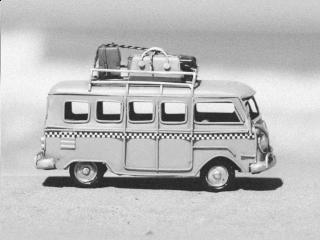
\includegraphics[width=0.3\textwidth]{figs/beachbus.jpg}
        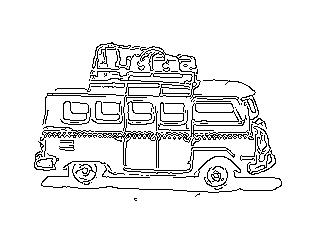
\includegraphics[width=0.3\textwidth]{figs/beachbus-canny.jpg}
\caption[Original image and post processed image]{Original image (A) and post-processed image (B).}
\label{fig:example} 
\end{figure}

You should add a copy of your code in the homework report as well:

\begin{lstlisting}[language=Python, caption=Python example]
import numpy as np
 
def incmatrix(genl1,genl2):
    m = len(genl1)
    n = len(genl2)
    M = None #to become the incidence matrix
    VT = np.zeros((n*m,1), int)  #dummy variable
 
    #compute the bitwise xor matrix
    M1 = bitxormatrix(genl1)
    M2 = np.triu(bitxormatrix(genl2),1) 
 
    for i in range(m-1):
        for j in range(i+1, m):
            [r,c] = np.where(M2 == M1[i,j])
            for k in range(len(r)):
                VT[(i)*n + r[k]] = 1;
                VT[(i)*n + c[k]] = 1;
                VT[(j)*n + r[k]] = 1;
                VT[(j)*n + c[k]] = 1;
 
                if M is None:
                    M = np.copy(VT)
                else:
                    M = np.concatenate((M, VT), 1)
 
                VT = np.zeros((n*m,1), int)
 
    return M
\end{lstlisting}

\newpage

% ----------------------------
% Section ends
% ============================

% ========================================================================================
%	Question 2
% ========================================================================================

\section{Part B}

\subsection{Profile Quick-sort}
\textbf{Description: For	this	problem	you	will	use	the	qsort.c	(quicksort)	program	provided,	and	you	
need	to	produce	a	dynamic	instruction	mix	table	(similar	to	Figure	A.29 in	your	
textbook)	to characterize	the	execution	of	the	quicksort	program. You	can	perform	
this	study	on	any	architecture	of	your	choice.	There	are	a	number	of approaches	you	
can	take	to	produce	this	data. Please	make	sure	to	explain	how	you	produced	the	data	in	your	table	and	provide
details	of	the	tools	that	you	used.}
\subsubsection{You	could	instrument	the	code	to	capture	the	execution	frequency	of	each
basic	block,	and	then,	using	an	assembly	listing	of	the	program,	provide
instruction	counts	(this	is	slightly	imprecise,	but	very	acceptable	for	this
assignment).}
\subsubsection{You	could	find	a	tracing	program	that	can	capture	an	instruction	trace.	You
would	then	have	to	write	a	program	to	count	individual	instructions
(challenging,	but	not	impossible).}
\subsubsection{You	could	find	a	tool	out	on	the	Internet	that	provides	this	capability	already
for	you.	While	this	sounds	easy,	it	may	be	a	bit	of	work	to	learn	the	particular
tool	you	have	chosen	to	use.}

\breakrule

\subsection{Solution}

% Sample text
This is where you write your answers. Adding a table as an example. You can reference it using this: Table~\ref{tab:example}.

\begin{table}[!htbp]
  \begin{center}
    \caption{Your first table.}
    \label{tab:example}
    \begin{tabular}{l|c|r} % <-- Alignments: 1st column left, 2nd middle and 3rd right, with vertical lines in between
      \textbf{Value 1} & \textbf{Value 2} & \textbf{Value 3}\\
      $\alpha$ & $\beta$ & $\gamma$ \\
      \hline
      1 & 1110.1 & a\\
      2 & 10.1 & b\\
      3 & 23.113231 & c\\
    \end{tabular}
  \end{center}
\end{table}

Adding a reference. The references are all in bib format. You can obtain these references from google scholar. Makes it a lot easier to add the references you need to cite on the homework. Just search for the paper you were reading on google scholar, and click on cite and search for the bibtex format. Add this reference (text) into the bib/sample.bib file and then cite the reference name inside this code. An example: Using the book~\cite{book} we answer the questions by providing Table~\ref{tab:example}. Tables can be generated with:
\lstinline{https://www.tablesgenerator.com/}.


\newpage

% ----------------------------
% Section ends
% ============================

% ========================================================================================
%	Question 3
% ========================================================================================

\section{Part C}

\subsection{Floating point benchmarks}
\textbf{Description: For	this	part	of	the	assignment,	write	two	different	benchmark	programs	on	your	
own that	contain significant	floating-point	content.		Compile	the	programs on	X86	
and	generate	an	assembly	listing	of the	benchmarks.		Then	identify	4 different	
floating-point	instructions	used	in	each program (a	total	of	8) and	explain	both	the	
operands	used	by	each	instruction	and	the	operation performed	on	the	operands	by	
the	instruction.}

\breakrule

\subsection{Solution}

\newpage

% ----------------------------
% Section ends
% ============================

% ========================================================================================
%	Question 4
% ========================================================================================

\section{Part D}

\subsection{Appendix K}
\textbf{Description: For	this	problem	you	will	need	to	read	through	Appendix	K	in	your	text,	covering	a	
number	of	instructions	sets,	and	then	answer	the	following	questions:}
\subsubsection{Name	2	CISC	instruction	set	architectures	and	2	RISC	instruction	set	
architectures.}
\subsubsection{Describe	3	characteristics	of	the	DEC	Alpha instruction	set.}
\subsubsection{Discuss	the	differences/similarities	between	MIPS	and	PowerPC	in	terms	of	
how	they	handle	conditional	branches.}
\subsubsection{Given	an	example	of	how	register	windows	work	on	the	SPARC	ISA.}
\subsubsection{In	your	opinion,	which	generation	of	the	Intel	x86	architecture	was	the	most	
significant	advancement	from	the	previous	generation	of	the	ISA.}

\breakrule

\subsection{Solution}


\newpage

% ----------------------------
% Section ends
% ============================

% ========================================================================================
%	Question 4
% ========================================================================================

\section{Part E}

\subsection{Amdahl}
\textbf{Description: Read	the	Amdahl,	Blaauw	and	Brooks	1964	paper	on	the	IBM	360	Architecture.
Given	the	timeframe	of	the	paper,	what	do	you	find	the	most	impressive	feature	of	
the	architecture	as	described	by	the	authors?		Justify	why	you	feel	this	is	such	a	
great	feature.		Also,	discuss the	representation	of	the	various	data types	supported	
on	this	important	ISA,	and	contrast	it	with	the	RISC-V.}

\breakrule

\subsection{Solution}


\newpage

% ----------------------------
% Section ends
% ============================

% ========================================================================================
%	Question 4
% ========================================================================================

\section{Part F}

\subsection{Chapter 1 Problems (Extra credit)}
\textbf{Description: Complete	problems	1.7,	1.8,	1.10,	and	1.12	(only	a	and	b) from	the	text.}

\breakrule

\subsection{Solution}


\newpage

% ----------------------------
% Section ends
% ============================

%----------------------------------------------------------------------------------------
%	BIBLIOGRAPHY
%----------------------------------------------------------------------------------------

\renewcommand{\refname}{\spacedlowsmallcaps{References}} % For modifying the bibliography heading

\bibliographystyle{plainnat}
\bibliography{bib/sample.bib} % The file containing the bibliography

%----------------------------------------------------------------------------------------

\end{document}